\documentclass[
11pt, % The default document font size, options: 10pt, 11pt, 12pt
%codirector, % Uncomment to add a codirector to the title page
]{charter} 

\usepackage{subfig}


% El títulos de la memoria, se usa en la carátula y se puede usar el cualquier lugar del documento con el comando \ttitle
\titulo{Autoencoders para reforzar modelos de prevención de fraude} 

% Nombre del posgrado, se usa en la carátula y se puede usar el cualquier lugar del documento con el comando \degreename
%\posgrado{Carrera de Especialización en Sistemas Embebidos} 
%\posgrado{Carrera de Especialización en Internet de las Cosas} 
\posgrado{Carrera de Especialización en Inteligencia Artificial}
%\posgrado{Maestría en Sistemas Embebidos} 
%\posgrado{Maestría en Internet de las cosas}

% Tu nombre, se puede usar el cualquier lugar del documento con el comando \authorname
\autor{Ariel Salassa} 

% El nombre del director y co-director, se puede usar el cualquier lugar del documento con el comando \supname y \cosupname y \pertesupname y \pertecosupname
\director{M. Sc. Lcdo. Franco Arito}
\pertenenciaDirector{Mercado Libre} 
% FIXME:NO IMPLEMENTADO EL CODIRECTOR ni su pertenencia
\codirector{John Doe} % para que aparezca en la portada se debe descomentar la opción codirector en el documentclass
\pertenenciaCoDirector{FIUBA}

% Nombre del cliente, quien va a aprobar los resultados del proyecto, se puede usar con el comando \clientename y \empclientename
\cliente{M. Sc. Lcdo. Franco Arito}
\empresaCliente{Mercado Libre}

% Nombre y pertenencia de los jurados, se pueden usar el cualquier lugar del documento con el comando \jurunoname, \jurdosname y \jurtresname y \perteunoname, \pertedosname y \pertetresname.
\juradoUno{Nombre y Apellido (1)}
\pertenenciaJurUno{pertenencia (1)} 
\juradoDos{Nombre y Apellido (2)}
\pertenenciaJurDos{pertenencia (2)}
\juradoTres{Nombre y Apellido (3)}
\pertenenciaJurTres{pertenencia (3)}
 
\fechaINICIO{24 de junio de 2021}		%Fecha de inicio de la cursada de GdP \fechaInicioName
\fechaFINALPlan{19 de agosto de 2021} 	%Fecha de final de cursada de GdP
\fechaFINALTrabajo{15 de junio de 2022}	%Fecha de defensa pública del trabajo final


\begin{document}

\maketitle
\thispagestyle{empty}
\pagebreak


\thispagestyle{empty}
{\setlength{\parskip}{0pt}
\tableofcontents{}
}
\pagebreak


\section*{Registros de cambios}
\label{sec:registro}


\begin{table}[ht]
\label{tab:registro}
\centering
\begin{tabularx}{\linewidth}{@{}|c|X|c|@{}}
\hline
\rowcolor[HTML]{C0C0C0} 
Revisión & \multicolumn{1}{c|}{\cellcolor[HTML]{C0C0C0}Detalles de los cambios realizados} & Fecha      \\ \hline
0.0      & Creación del documento                                 			& 24/06/2021 \\ \hline
1.0      & Se completa hasta la sección 5 inclusive               	& 07/07/2021 \\ \hline
1.1      & Correcciones de la versión 1.0                 					& 08/07/2021 \\ \hline
2.0      & Se completa hasta la sección 9 inclusive					& 14/07/2021 \\ \hline
2.1      & Correcciones de la versión 1.0 									& 22/07/2021 \\ \hline
3.0      & Se completa hasta la sección 12 inclusive					& 29/07/2021 \\ \hline
%		  Se puede agregar algo más \newline
%		  En distintas líneas \newline
%		  Así                                                    & dd/mm/aaaa \\ \hline
%3      & Se completa hasta el punto 11 inclusive                & dd/mm/aaaa \\ \hline
%4      & Se completa el plan	                                 & dd/mm/aaaa \\ \hline
\end{tabularx}
\end{table}

\pagebreak



\section*{Acta de constitución del proyecto}
\label{sec:acta}

\begin{flushright}
Buenos Aires, \fechaInicioName
\end{flushright}

\vspace{2cm}

Por medio de la presente se acuerda con el Ing. \authorname\hspace{1px} que su Trabajo Final de la \degreename\hspace{1px} se titulará ``\ttitle'' y  consistirá esencialmente en un sistema que aporte información complementaria para el entrenamiento de futuros modelos de prevención de fraude de pagos electrónicos. El Trabajo Final tendrá un presupuesto preliminar estimado de 600 hs de trabajo y recursos económicos brindados por la empresa Mercado Libre, con fecha de inicio \fechaInicioName\hspace{1px} y fecha de presentación pública \fechaFinalName.

Se adjunta a esta acta la planificación inicial.

\vfill

% Esta parte se construye sola con la información que hayan cargado en el preámbulo del documento y no debe modificarla
\begin{table}[ht]
\centering
\begin{tabular}{ccc}
\begin{tabular}[c]{@{}c@{}}Ariel Lutenberg \\ Director posgrado FIUBA\end{tabular} & \hspace{2cm} & \begin{tabular}[c]{@{}c@{}}\clientename \\ \empclientename \end{tabular} \vspace{2.5cm} \\ 
\multicolumn{3}{c}{\begin{tabular}[c]{@{}c@{}} \supname \\ Director del Trabajo Final\end{tabular}} \vspace{2.5cm} \\
%\begin{tabular}[c]{@{}c@{}}\jurunoname \\ Jurado del Trabajo Final\end{tabular}     &  & \begin{tabular}[c]{@{}c@{}}\jurdosname\\ Jurado del Trabajo Final\end{tabular}  \vspace{2.5cm}  \\
%\multicolumn{3}{c}{\begin{tabular}[c]{@{}c@{}} \jurtresname\\ Jurado del Trabajo Final\end{tabular}} \vspace{.5cm}                                                                     
\end{tabular}
\end{table}




\section{1. Descripción técnica-conceptual del proyecto a realizar}
\label{sec:descripcion}

Mercado Pago es la plataforma fintech dentro del ecosistema de Mercado Libre (Meli). En esta plataforma, que tiene millones de usuarios activos, se ofrecen distintas soluciones tecnológicas que hace posible pagar y cobrar en forma online. Algunos ejemplos de dichas soluciones son: abono de servicios, recargas de teléfono o pases de transporte, pagos y cobros con códigos QR, envíos de dinero, entre otros.

Dada la gran cantidad de usuarios y transacciones, y la variedad de estas, ha sido necesario desarrollar modelos de machine learning que sean capaces de detectar transacciones fraudulentas que perjudican reputacional y económicamente  a la empresa, como se puede visualizar en la Figura \ref{fig:fraudster}.

\begin{figure}[H]
\centering
\frame{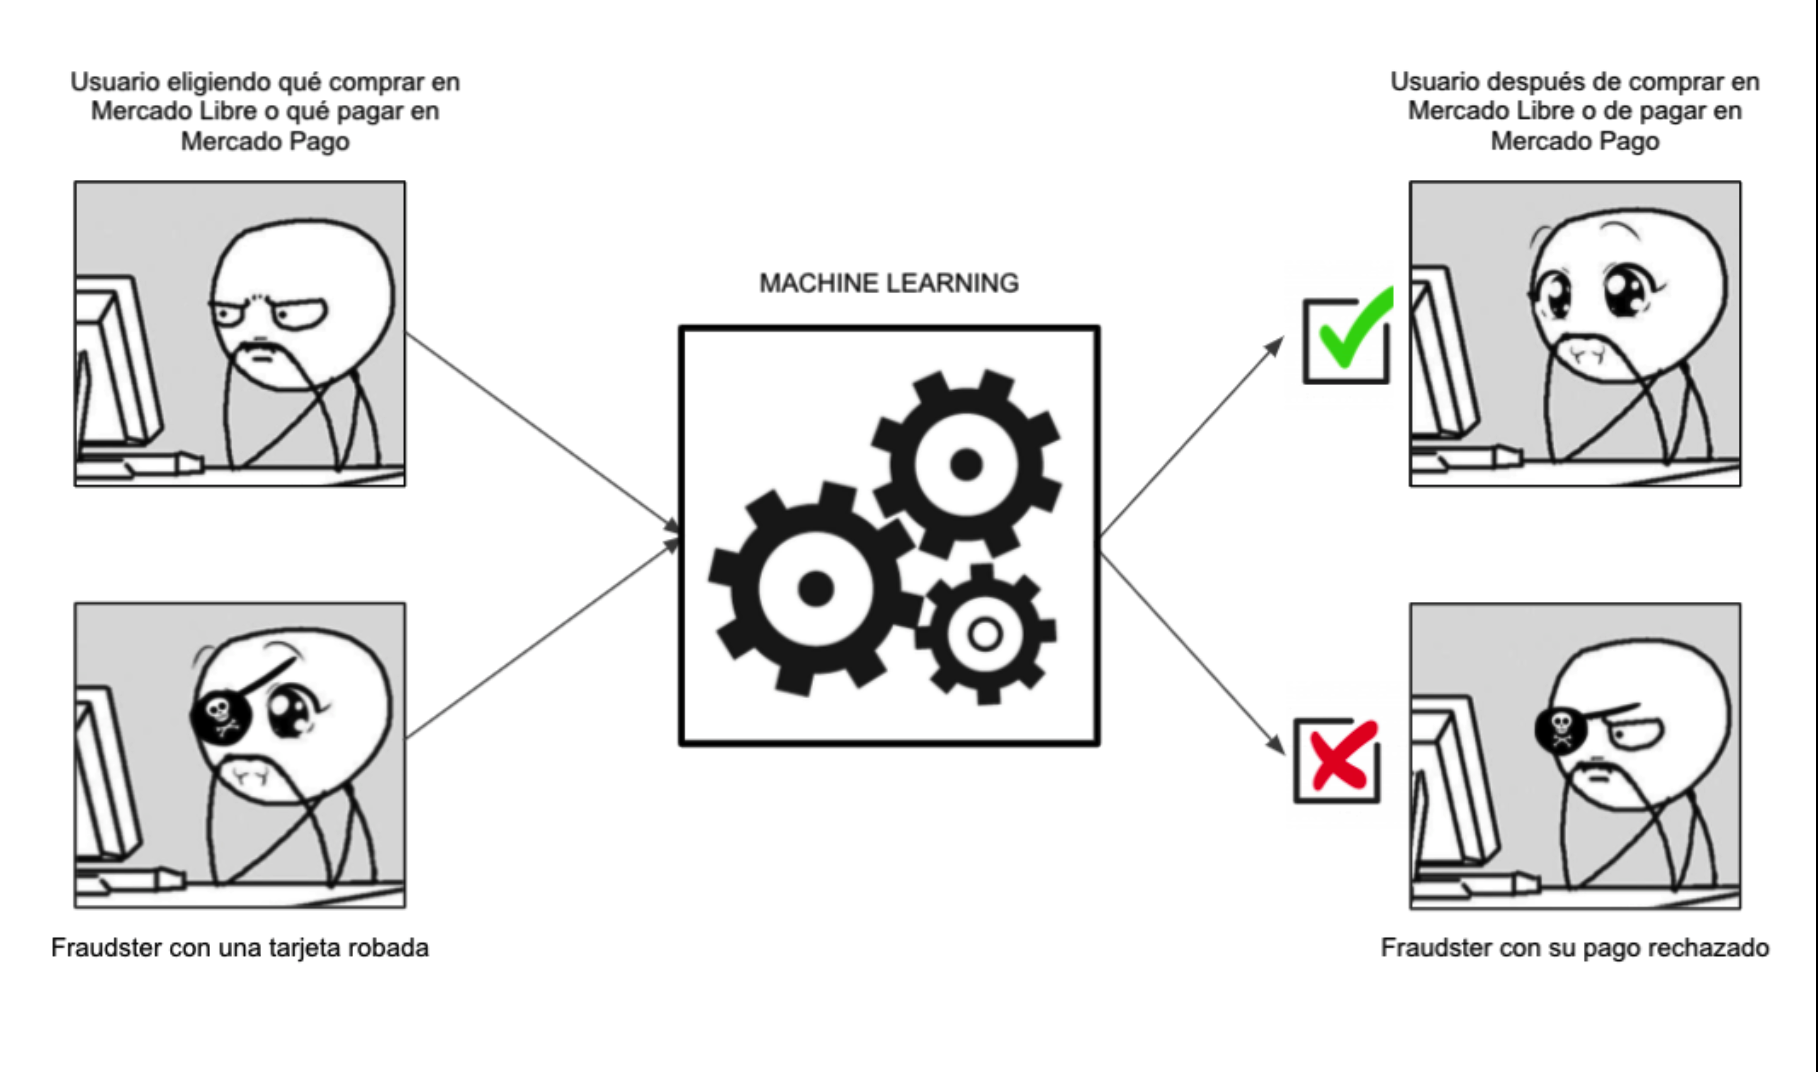
\includegraphics[width=.9\textwidth]{./Figuras/fraudster.png}}
\caption{Esquema del comportamiento esperado de los usuarios dentro de las plataformas de Meli.}
\label{fig:fraudster}
\end{figure}

El entrenamiento de modelos de machine learning para este tipo de aplicaciones conlleva una dificultad adicional: los datos de entrenamiento están fuertemente desbalanceados, es decir, la cantidad de pagos no fraudulentos es mucho mayor que la cantidad de pagos fraudulentos.

Para hacerle frente a este problema, lo que se propone hacer es entrenar un autoencoder, cuya arquitectura esquemática se muestra en la Figura \ref{fig:autoencoder}, sólo con pagos fraudulentos. De esta manera será posible enriquecer los registros de pagos que en el pasado fueron rechazados por ser riesgosos para poder tomarlos en cuenta en futuros entrenamientos. 

Por otro lado, el autoencoder presenta en su capa central o capa latente una representación reducida y codificada de la entrada. Es de esperarse que a partir de ella puedan visualizarse patrones de fraudes conocidos y, eventualmente, sacar conclusiones o indicios de patrones de fraudes sin conocer. El potencial de dicha representación puede verse en la Figura \ref{fig:latentRepresentation}.

\begin{figure}[H]
\centering
\frame{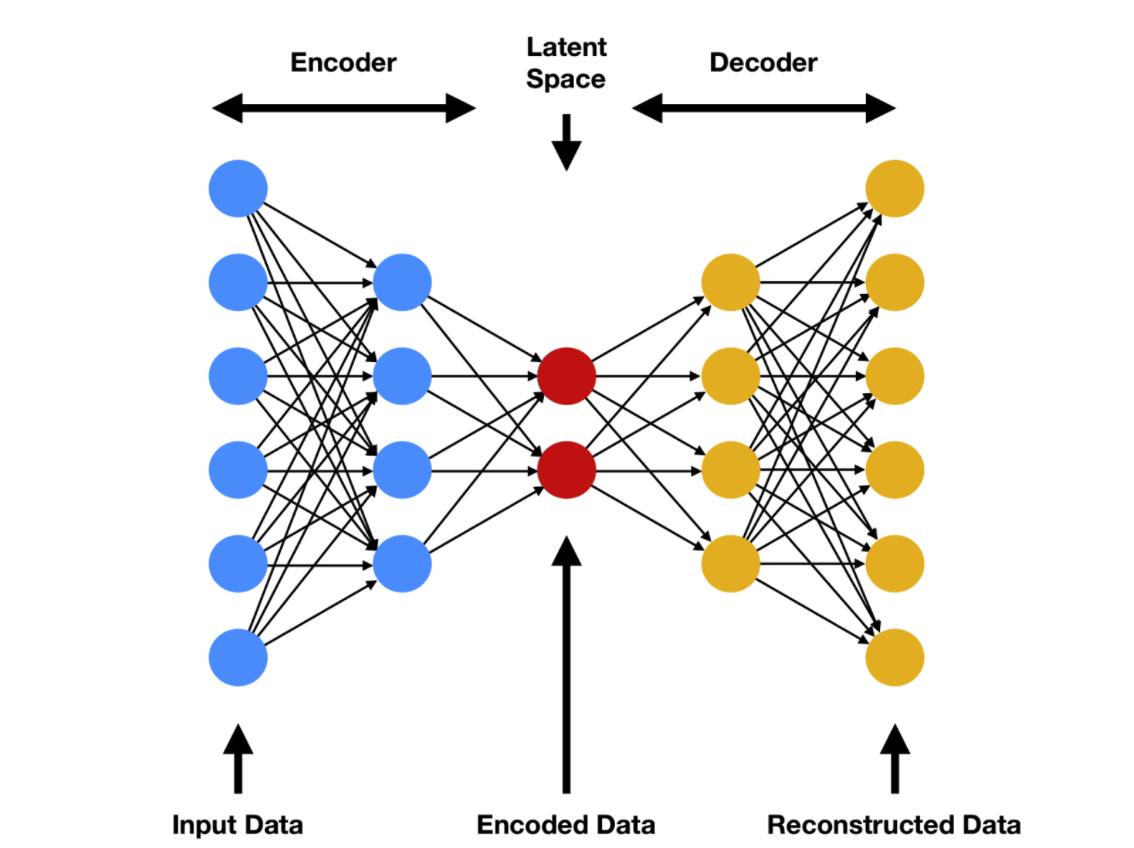
\includegraphics[width=.6\textwidth]{./Figuras/autoencoder.png}}
\caption{Arquitectura representativa de un autoencoder.}
\label{fig:autoencoder}
\end{figure}

\begin{figure}[H]
\centering
\subfloat[Descomposición de datos de entrada.]{\frame{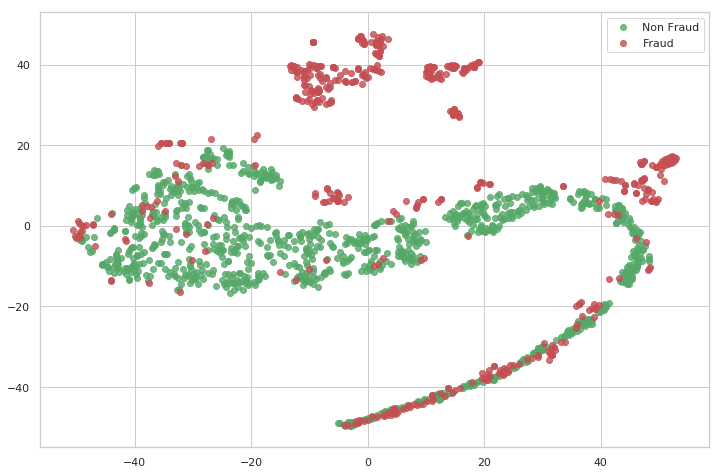
\includegraphics[width=0.47\textwidth]{./Figuras/actualRepr.png}}}
\hspace{0.05\textwidth}
\subfloat[Descomposición de datos latentes.]{\frame{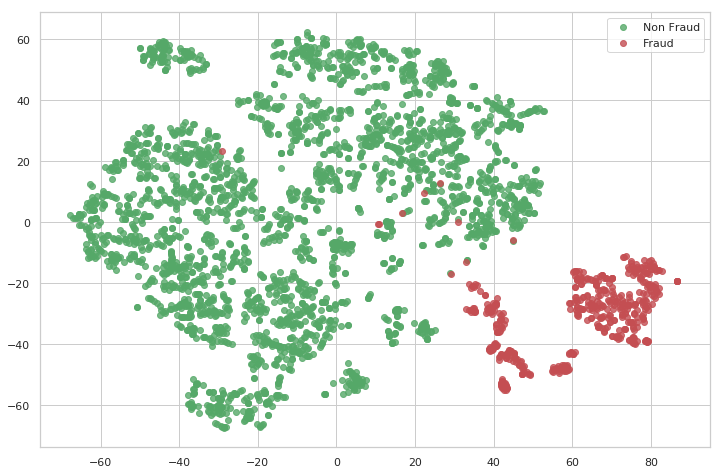
\includegraphics[width=0.47\textwidth]{./Figuras/latentRepr.png}}}
%\frame{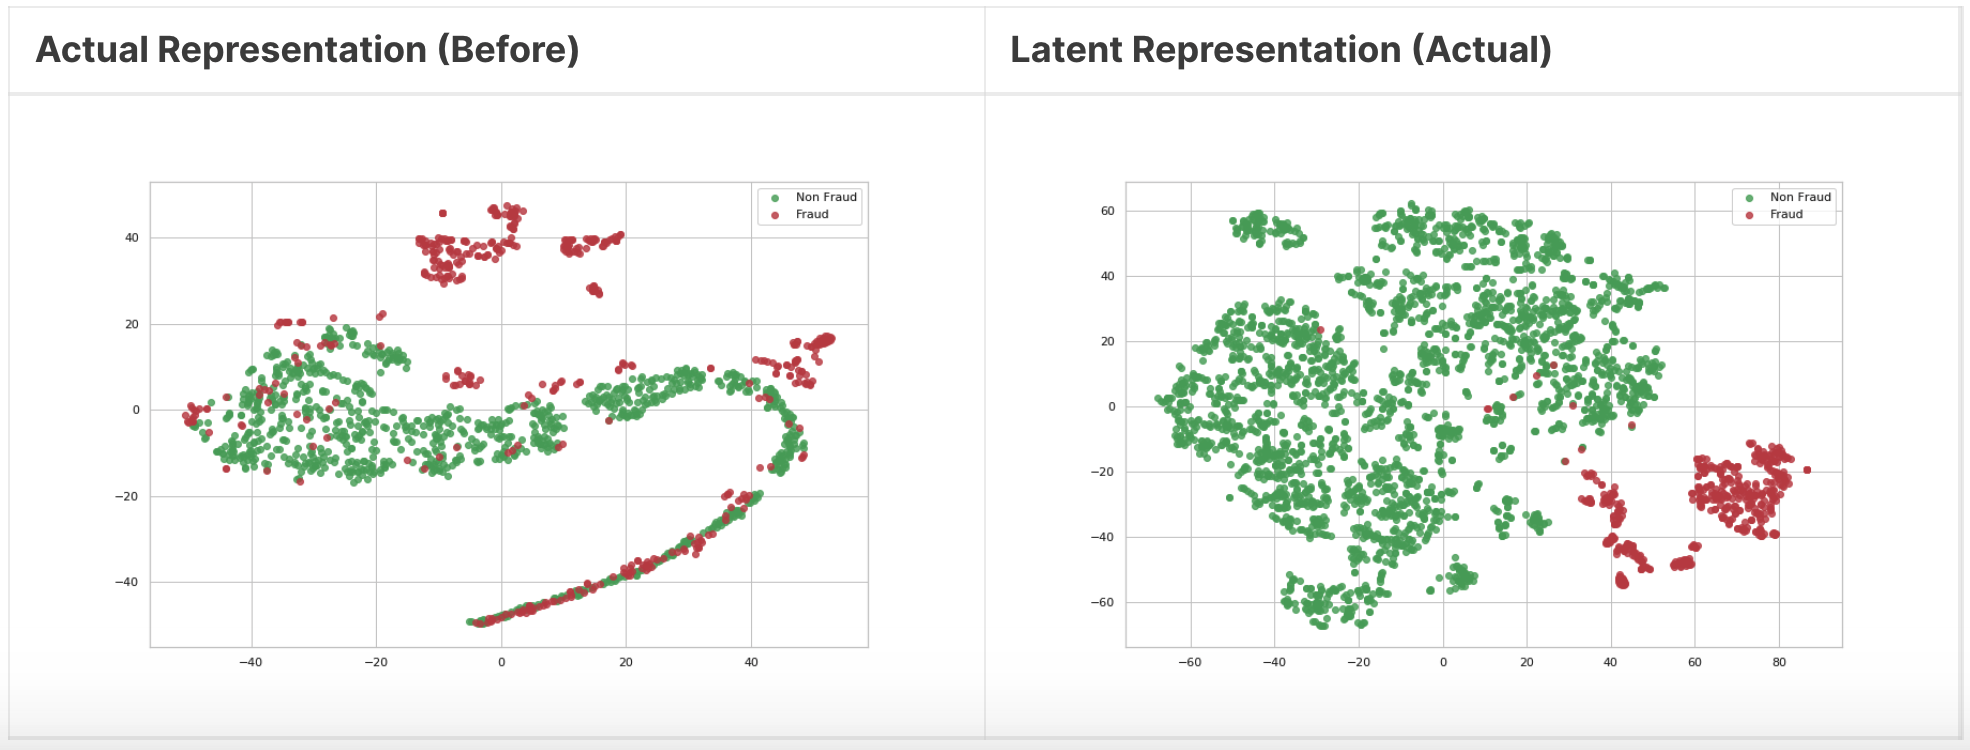
\includegraphics[width=\textwidth]{./Figuras/latentRepresentation.png}}
\caption{Imagen ilustrativa del artículo \emph{‘Semi Supervised Classification using AutoEnconders’} de Kaggle usando el método de descomposición T-SNE (\emph{t-Distributed Stochastic Neighbor Embedding}) aplicado a los datos.}
\label{fig:latentRepresentation}
\end{figure}

En la Figura \ref{fig:esquemaSistema} se observa un diagrama de bloques que ilustra cómo sería el funcionamiento del sistema en producción. En primer lugar, un usuario realizaría un pago en línea. Inmediatamente, el pago entra al sistema y se obtiene una representación vectorizada del mismo con los atributos de interés. Esta codificación del pago pasa por la red neuronal del motor de fraude y se obtiene una probabilidad de que el pago sea fraudulento (predicción). En función de la probabilidad de fraude y otros factores se decide si el pago se rechaza o se aprueba y se guardan todos los valores en una base de datos. En caso de que el pago sea rechazado, el mismo se envía al autoencoder de Fraude. Del autoencoder se obtendrá una puntuación de fraude asociada al pago rechazado que también se guardará en la base de datos. 

La puntuación de fraude será una medida de la capacidad de reconstrucción del autoencoder y  representará qué tan similar a un fraude real es el pago rechazado. Al momento de entrenar nuevos modelos de red o reentrenar modelos existentes, los pagos con alta puntuación podrán ser considerados en el dataset de entrenamiento. 

\begin{figure}[htpb]
\centering
\frame{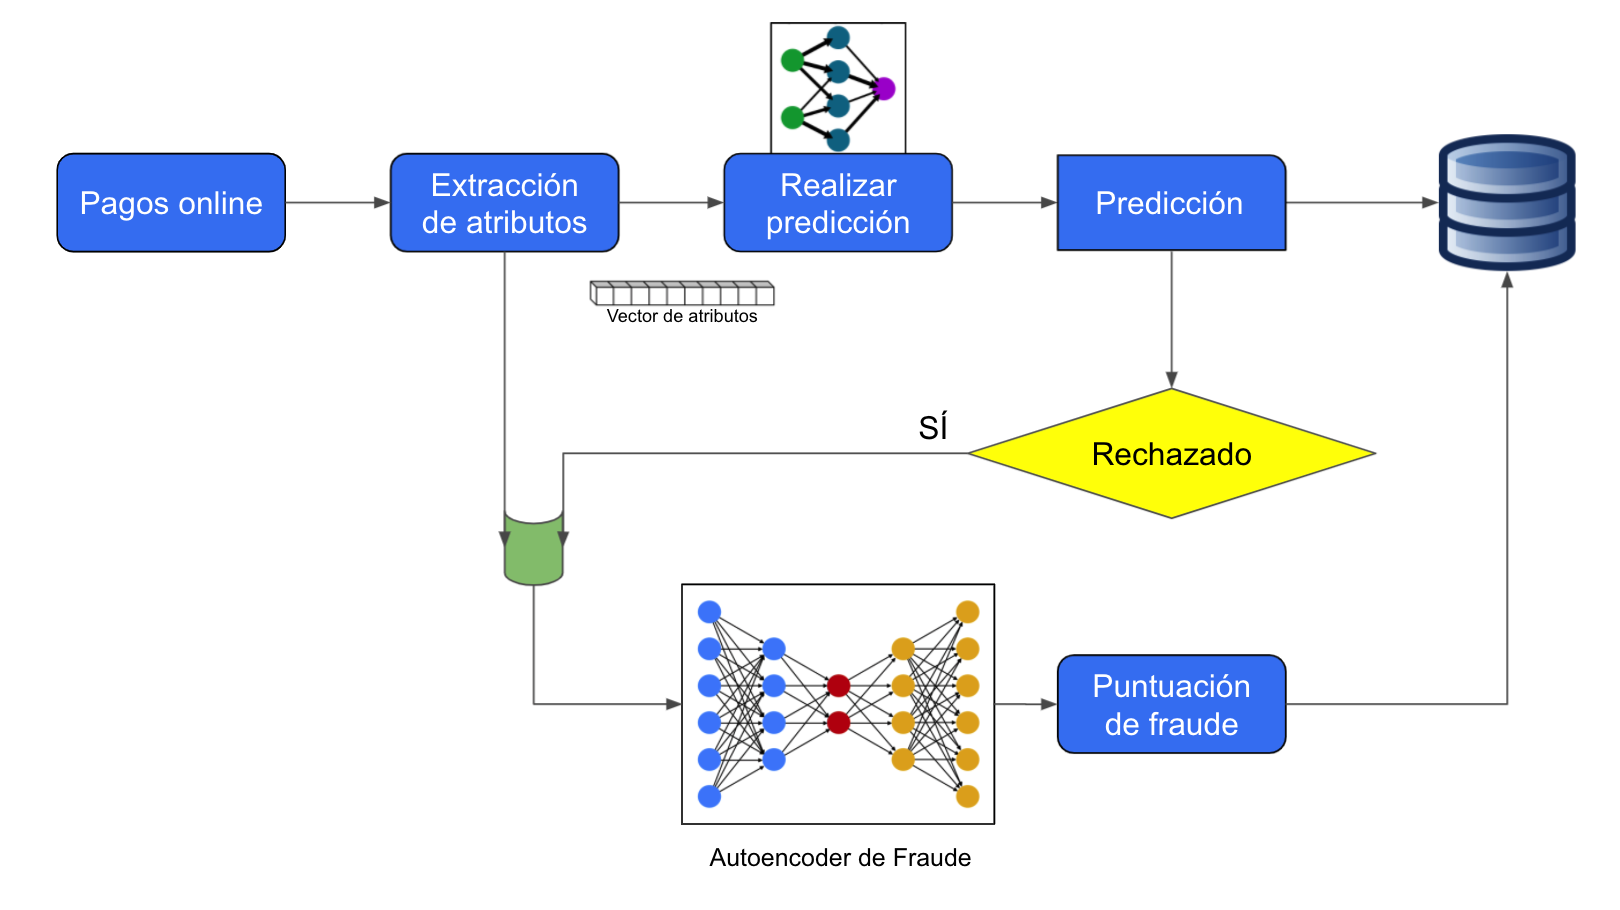
\includegraphics[width=\textwidth]{./Figuras/esquemaSistema.png}}
\caption{Diagrama de bloques del funcionamiento del sistema.}
\label{fig:esquemaSistema}
\end{figure}

\section{2. Identificación y análisis de los interesados}
\label{sec:interesados}

\begin{table}[ht]
\begin{tabularx}{\linewidth}{@{}|l|X|l|X|@{}}
\hline
\rowcolor[HTML]{C0C0C0} 
Rol           & Nombre y Apellido & Organización 	& Puesto 	\\ \hline
Responsable   & \authorname       & Mercado Libre   & ML Engineer \newline Alumno 	\\ \hline
Colaboradores & Ing. Paz Martin \newline 
    							Lcdo. Joaquín Loyola \newline 
    							Ing. Enrique Serdio    
    						& Mercado Libre  
    						& Sr. Data Scientist \newline 
    							Sr. Data Engineer \newline 
    							Sr. ML Engineer		\\ \hline
Orientador    & \supname	      & \pertesupname 	& Sr. ML Expert \newline Director Trabajo final \\ \hline
Usuario final & Desarrolladores de Machine Learning & Mercado Libre   & Data Scientists \newline ML Engineers       	\\ \hline
\end{tabularx}
\caption{Identificación de los interesados}
\label{tab:interesados}
\end{table}

\begin{itemize}
	\item Responsable: \authorname, es la persona que desarrollará el proyecto.
	\item Colaboradores:
	\begin{itemize}
        \item{Paz Martín}: es líder y referente técnica del equipo de científicos de datos donde se desempeña el responsable. Validará la gestión del tiempo y será capaz de orientar en el desarrollo si el responsable lo requiriese. 
        \item{Joaquín Loyola}: es líder y referente técnico del equipo de ingeniería de datos. Su colaboración pasará por asistir al referente en cuestiones ligadas a los datos de entrenamiento, si fuese necesario.
        \item{Enrique Serdio}: es referente técnico del equipo de ML Ops. Su colaboración se centrará, si fuese necesario, en asistir al responsable en cuestiones ligadas a la infraestructura de los modelos de machine learning en la nube.
      \end{itemize}
	\item Orientador: Franco Arito es el director del presente proyecto y líder técnico de múltiples equipos de Mercado Libre. Su función será orientar al responsable a lo largo de la realización del proyecto.
	\item Desarrolladores de Machine Learning: son los usuarios finales que podrán hacer uso del sistema para enriquecer sus modelos.
\end{itemize}

\section{3. Propósito del proyecto}
\label{sec:proposito}
El propósito de este proyecto es poner en valor los pagos que son rechazados por el motor de fraude y que tienen potencial de ser utilizados en futuros entrenamientos de redes neuronales de manera tal de reducir el desbalance de los datasets de entrenamiento y validación. Además, se espera que la representación en la capa latente permita evaluar oportunidades para determinar perfiles de fraude. Con una representación como esta, los equipos de prevención tendrán a su disposición una herramienta que les permitirá ser más reactivos ante posibles ataques. 

\section{4. Alcance del proyecto}
\label{sec:alcance}
El proyecto comprenderá las siguientes etapas:
\begin{itemize}
\item Planificación de tareas.
\item Formación en TensorFlow.
\item Investigación de autoencoders aplicados a la prevención de fraude.
\item Selección y extracción del dataset para realizar prueba de concepto del modelo.
\item Análisis de datos del dataset.
\item Pruebas de arquitectura de red.
\item Visualización y análisis de datos de la capa latente utilizando el método de descomposición T-SNE.
\item Evaluación de distintas formas de hacer etiquetado (labeling).
\item Evaluación de la performance del sistema comparado con otras soluciones.
\item Evaluación del modelo con otros datasets.
\end{itemize}


El presente proyecto no incluye:
\begin{itemize}
\item Aplicación de algoritmos de clustering para los datos codificados a partir de la capa latente.
\item Despliegue del modelo y puesta en producción.
\end{itemize}


\section{5. Supuestos del proyecto}
\label{sec:supuestos}
Para el desarrollo del presente proyecto se supone que:
\begin{itemize}
	\item El responsable dispondrá de suficiente cantidad de tiempo para encarar los problemas que se presenten en el desarrollo del proyecto.
	\item El responsable tendrá a su disposición a su director y/o colaboradores cuando sea pertinente.
	\item TensorFlow es el framework de cálculo numérico que dispone de todas las herramientas necesarias para encarar este proyecto.
	\item El autoencoder entrenado solamente con pagos fraudulentos tendrá buen ratio de reconstrucción de datos a la hora de evaluar pagos rechazados por alto riesgo.
	\item La puntuación de Fraude (asociada con la medida de reconstrucción de un pago) será un dato de tipo flotante, o bien, un dato de tipo categórico basado en ciertos valores de corte (thresholds). 
	\item Es posible aplicar el método de descomposición T-SNE a los datos codificados y, a partir de su representación en dos o tres dimensiones, se podrán realizar nuevos análisis, por ejemplo, la identificación de clusters de fraudes.
	\item Una vez que el autoencoder esté entrenado y validado con un set de pagos, su aplicación podrá generalizarse.
	\item El comportamiento de los usuarios que provocan el fraude no mutará mientras tiene lugar el desarrollo de este proyecto.
\end{itemize}

\section{6. Requerimientos}
\label{sec:requerimientos}

\begin{enumerate}
	\item Requerimientos de documentación
		\begin{enumerate}
			\item Toda documentación compartida debe mantenerse dentro de un acuerdo de confidencialidad.
			\item El trabajo debe ser continuamente documentado y se presentarán informes de avance una vez cada tres semanas al director.
			\item Los informes de avance pueden ser presentados como código correctamente documentado con los resultados correspondientes.
		\end{enumerate}
	\item Requerimientos de forma trabajo
		\begin{enumerate}
			\item Se utilizará una metodología de trabajo ágil e iterativa con mucha interacción entre el responsable, el director y los colaboradores.
		\end{enumerate}
	\item Requerimientos de lenguajes y frameworks
		\begin{enumerate}
			\item Los datos deberán ser consultados a base de datos relacionales. El lenguaje para estas transacciones debe ser SQL y debe ser lo más agnóstico posible intentando de no usar funciones que sean específicas de uno y otro proveedor.
			\item El framework utilizado debe ser Tensor Flow en su versión V2.0 o superior en Python.
			\item Todo análisis debe realizarse en código Python dentro de Jupyter labs y utilizando librerías standard  (numpy, pandas, matplotlib, seaborn, etcétera).
		\end{enumerate}
	\item Requerimientos de infraestructura
		\begin{enumerate}
			\item Las queries de extracción de datos deben ser compatibles con Amazon Redshift y/o Google BigQuery.
			\item Los datasets deben ser guardados en Amazon S3 o Google Cloud Storage como archivos con extensión \emph{.csv}.
			\item En caso de ser necesario un hardware específico de entrenamiento, deberán usarse los servicios de Google Cloud Platform (GCP).
		\end{enumerate}
	\item Requerimientos funcionales
		\begin{enumerate}
			\item La extracción de datos no puede demorar más de 24 hs.
			\item El modelo entrenado debe tener una precisión de al menos 85\%.
			\item El modelo debe ser entrenado con al menos diez mil registros.
			\item El entrenamiento del modelo no puede demorar más de 24 hs.
			\item El tipo de dato que represente la puntuación de fraude debe ser categórico o flotante.
			\item Las representaciones resultantes de la descomposición deben poder visualizarse en dos o tres dimensiones.
		\end{enumerate}
	\item Requerimientos de testing y evaluación
		\begin{enumerate}
			\item La efectividad de la puntuación de fraude debe ser evaluada contra una marca dada por una heurística conocida.
			\item Dicha puntuación debe ser igual o mejor que dicha marca.
		\end{enumerate}
\end{enumerate}

\section{7. Historias de usuarios (\textit{Product backlog})}
\label{sec:backlog}
La medida del trabajo a efectuar para cumplir con cada una de las historias de usuarios estará dada por \emph{story points}. Para ponderar los esfuerzos se utilizará la serie de Fibonacci con valores: 0, 1, 2, 3, 5, 8, 13, 21, 34, 55, 89, etc. Cuando el esfuerzo se considere alto los \emph{story points} tomarán valores entre 0 y 3 inclusive. Cuando se considere medio, entre 5 y 13 inclusive. Cuando el esfuerzo se considere alto el valor de los \emph{story points} será igual o mayor a 21.

\begin{itemize}
\item Como analista y desarrollador quiero una métrica de fraude para reutilizar pagos rechazados por alto riesgo en futuros entrenamientos y futuros análisis. 

Dificultad: Alta (34) -- Complejidad: Alta (34)  -- Incertidumbre: Alta (34)

Story Points: 34 + 34 + 34 = 102 $\rightarrow$ 89

\item Como cliente quiero tener un modelo de red realizado con tecnologías standards y \emph{open source} para poder mantenerlo a futuro con el menor esfuerzo posible.

Dificultad: Media (8) -- Complejidad: Media (8) -- Incertidumbre: Baja (1)

Story Points: 8 + 8 + 1 = 17 $\rightarrow$ 21

\item Como analista de datos quiero tener una representación simplificada del fraude para entender posibles ataques y ser reactivo en consecuencia.

Dificultad: Alta (21)  -- Complejidad: Alta (21) -- Incertidumbre: Alta (21)

Story Points: 21 + 21 + 21 = 63 $\rightarrow$  55

\item Como cliente quiero tener las bases de un modelo de red preciso para servirlo en producción adaptándose a flujos preexistentes.

Dificultad: Media (8) -- Complejidad: Media (8) -- Incertidumbre: Alta (21)

Story Points: 8 + 8 + 21 = 37 $\rightarrow$ 34

\item Como cliente quiero recibir la documentación del trabajo realizado para que pueda servir como base de futuros desarrollos de la empresa.

Dificultad: Media (13) -- Complejidad: Baja (2) -- Incertidumbre: Baja (1)

Story Points: 13 + 2 + 1 = 16 $\rightarrow$ 13

\item Como cliente quiero tener una presentación resumida del trabajo para mostrar sus resultados y su potencial potencial a todos los interesados.

Dificultad: Baja (3) -- Complejidad: Baja (2) -- Incertidumbre: Baja (2)

Story Points: 3 + 2 + 2 = 7 $\rightarrow$ 8


\end{itemize}

\section{8. Entregables principales del proyecto}
\label{sec:entregables}

Los entregables del proyecto que conservará la empresa donde trabaja el responsable y el director son:

\begin{itemize}
 \item Informe final.
 \item Presentación final.
 \item Datasets utilizados.
 \item Queries de extracción documentadas.
 \item Jupyter labs de análisis documentados.
\end{itemize}

Además, se entregará a los docentes responsables de la Carrera de Especialización en Inteligencia Artificial de la UBA el informe final del proyecto con firma previa de los documentos de confidencialidad.

\section{9. Desglose del trabajo en tareas}
\label{sec:wbs}


\begin{enumerate}
\item Planificación (60 hs)
	\begin{enumerate}
		\item Estudio de necesidades (9 hs)
		\item Análisis de factibilidad (3 hs)
		\item Definición de requerimientos (9 hs)
		\item Confección de documento de planificación (39 hs)
	\end{enumerate}
\item Investigación y capacitación (114 hs)
	\begin{enumerate}
		\item Estudio de distintos tipos de autoencoders (9 hs)
		\item Estudio de autoencoders aplicados a la prevención de fraude (3 hs)
		\item Capacitación en Tensor Flow 2 (15 hs)
		\item Capacitación en \emph{feature preprocessing} y \emph{feature engineering} (24 hs)
		\item Capacitación en \emph{feature selection} (15 hs)
		\item Capacitación en SQL aplicado a Amazon Redshift y Google BigQuery (9 hs)
		\item Capacitación en \emph{Machine Learning pipelines} en GCP (15 hs)
		\item Estudio de algoritmo T-SNE (9 hs)
		\item Elaboración de códigos de ejemplos básicos (15 hs)
	\end{enumerate}
\item Confección dataset de prueba (45 hs)
	\begin{enumerate}
		\item Exploración y elección tablas (9 hs)
		\item Análisis de completitud de datos (9 hs)
		\item Confección de query de extracción (9 hs)
		\item Extracción de datos (3 hs)
		\item Selección de features (15 hs)
	\end{enumerate}
\item Entrenamiento (78 hs)
	\begin{enumerate}
		\item Aplicación de \emph{feature preprocessing} (15 hs)
		\item Prueba de distintas arquitecturas de red con distintas configuraciones (39 hs)
		\item Evaluación y ajuste del modelo (24 hs)
	\end{enumerate}
\item Pruebas de validación (63 hs)
	\begin{enumerate}
		\item Evaluación de distintas estrategias de \emph{labeling} (39 hs)
		\item Comparación de resultados en función de heurísitcas conocidas (24 hs)
	\end{enumerate}
\item Representación reducida (63 hs)
	\begin{enumerate}
 		\item Visualización de datos de la capa de entrada utilizando el método de descomposición T-SNE (15 hs)
 		\item Visualización de datos de la capa latente utilizando el método de descomposición T-SNE (15 hs)
 		\item Visualización segmentada de los datos en función de features de interés del modelo (33 hs)
 	\end{enumerate}
\item Generalización (87 hs)
 	\begin{enumerate}
 		\item Extracción de datos correspondientes a otro flujo de datos (24 hs)
 		\item Análisis de completitud de datos (15 hs)
 		\item Comparación y análisis de resultados (24 hs)
 		\item Ajustes finales (24 hs)
 	\end{enumerate}
\item Documentación y presentación final (90 hs)
 	\begin{enumerate}
 		\item Elaborar informe final del proyecto (50 hs)
 		\item Preparación de presentación final (30 hs)
 	\end{enumerate}
\end{enumerate}

Cantidad total de horas: (600 hs)

\section{10. Diagrama de Activity On Node}
\label{sec:AoN}

En la Figura \ref{fig:aon} se muestra el diagrama de \emph{Activity on Node} del proyecto. Las flechas resaltadas en negro ilustran el camino crítico del proyecto. También se puede ver que los hitos marcan el fin de las distintas fases del proyecto, las cuales, a su vez, están representadas en distintos colores.

\begin{figure}[htpb]
\centering 
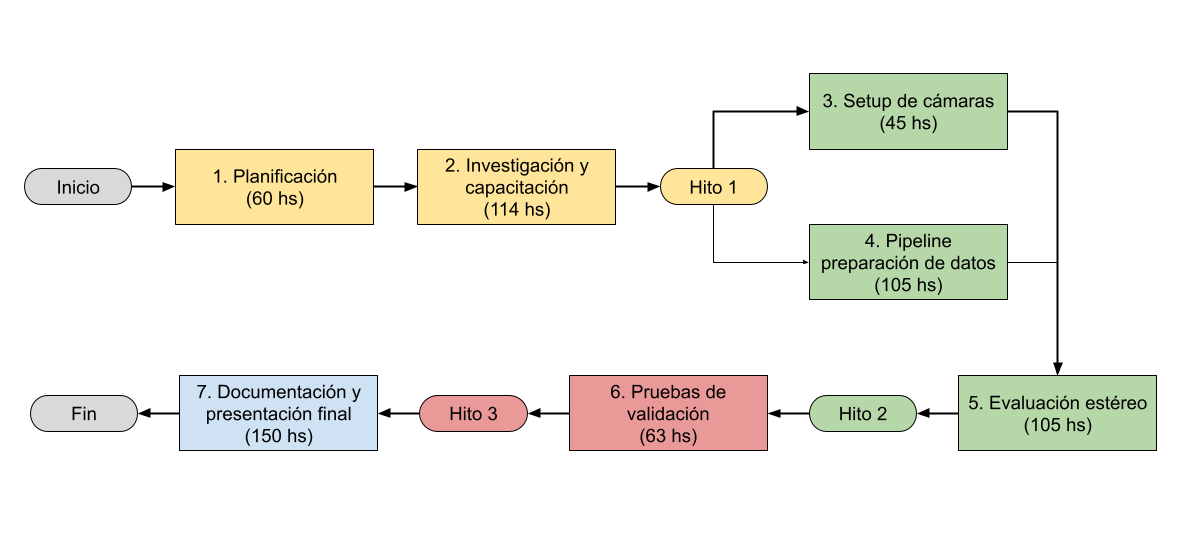
\includegraphics[width=\textwidth]{./Figuras/aon.png}
\caption{Diagrama en \textit{Activity on Node.}}
\label{fig:aon}
\end{figure}

\section{11. Diagrama de Gantt}
\label{sec:gantt}

A continuación se muestra el diagrama de Gant del presente proyecto. Se consideró la jornada laboral de 3 horas de trabajo desde la fecha de inicio del curso hasta finales de abril del próximo año.
En la figura \ref{fig:ganttReducido} y \ref{fig:ganttCompleto} se muestra el diagrama de Gantt de forma compacta y de forma desglosada respectivamente, tal como se enumeró en la sección 9.

\begin{figure}[htpb]
\centering 
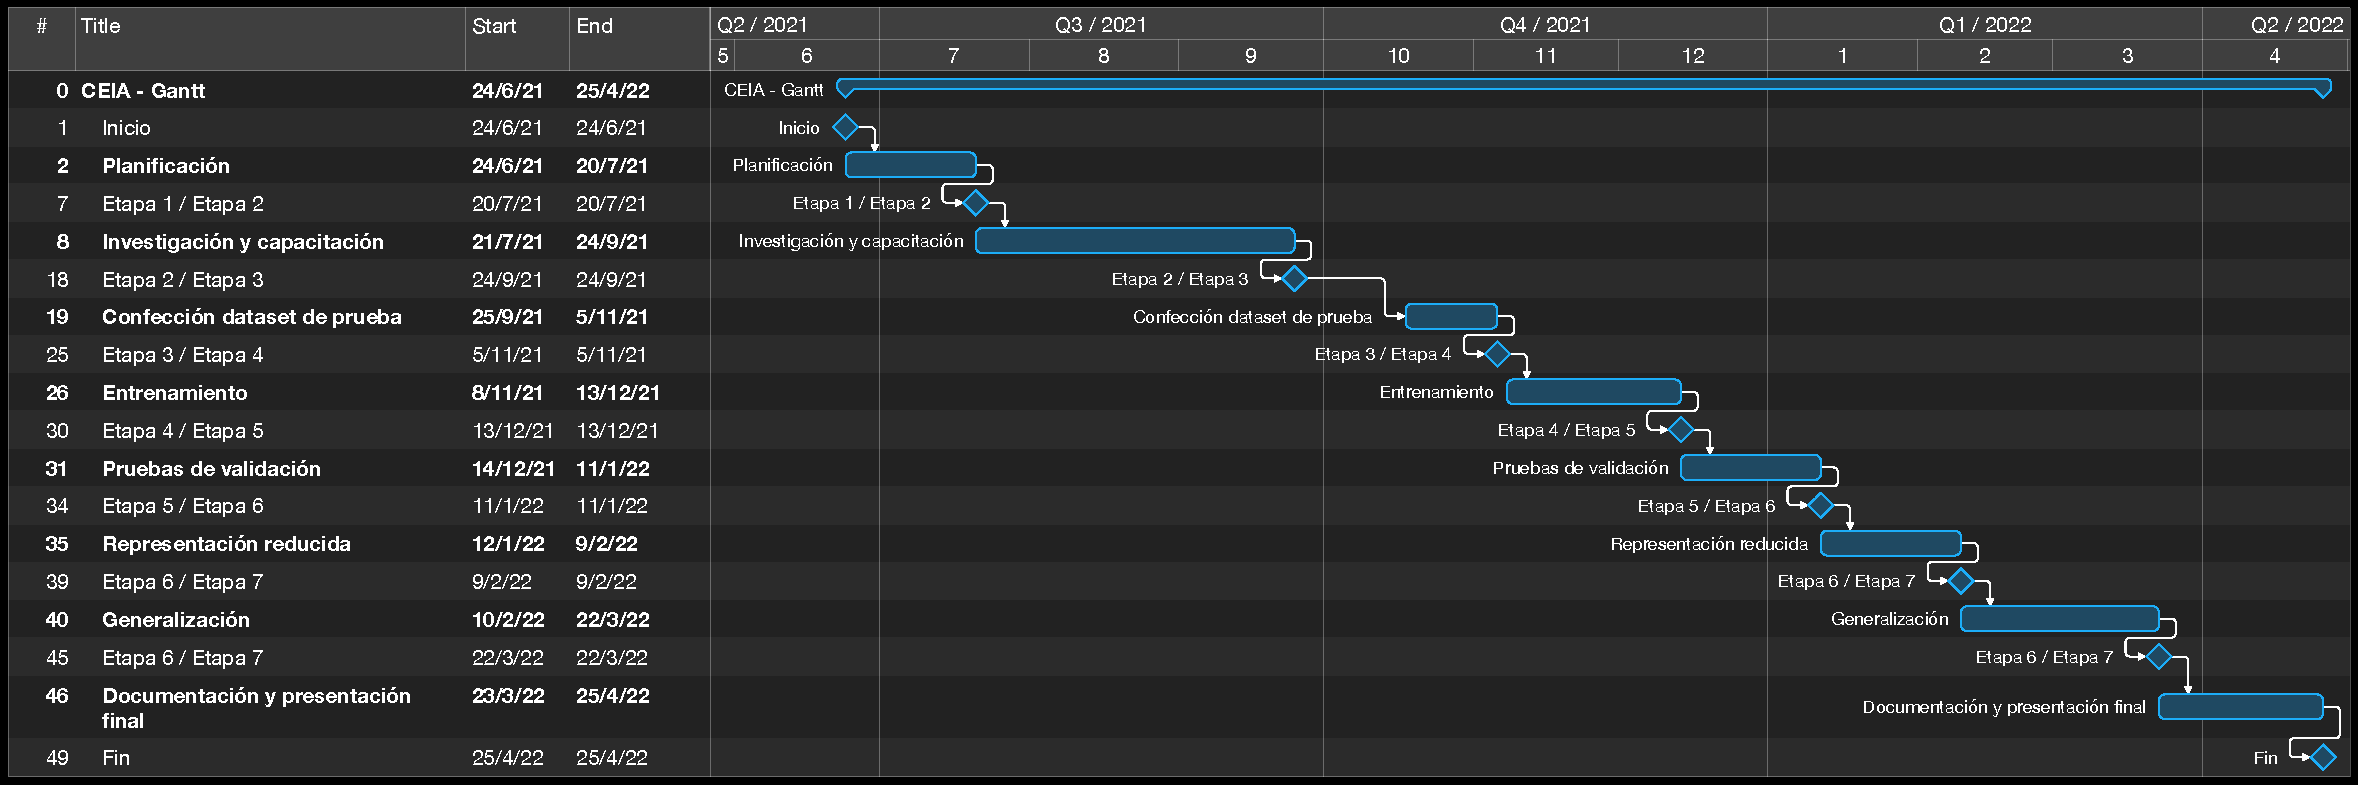
\includegraphics[width=\textwidth]{./Figuras/ganttReducido.pdf}
\caption{Diagrama de Gantt reducido.}
\label{fig:ganttReducido}
\end{figure}

\begin{figure}[htpb]
\centering 
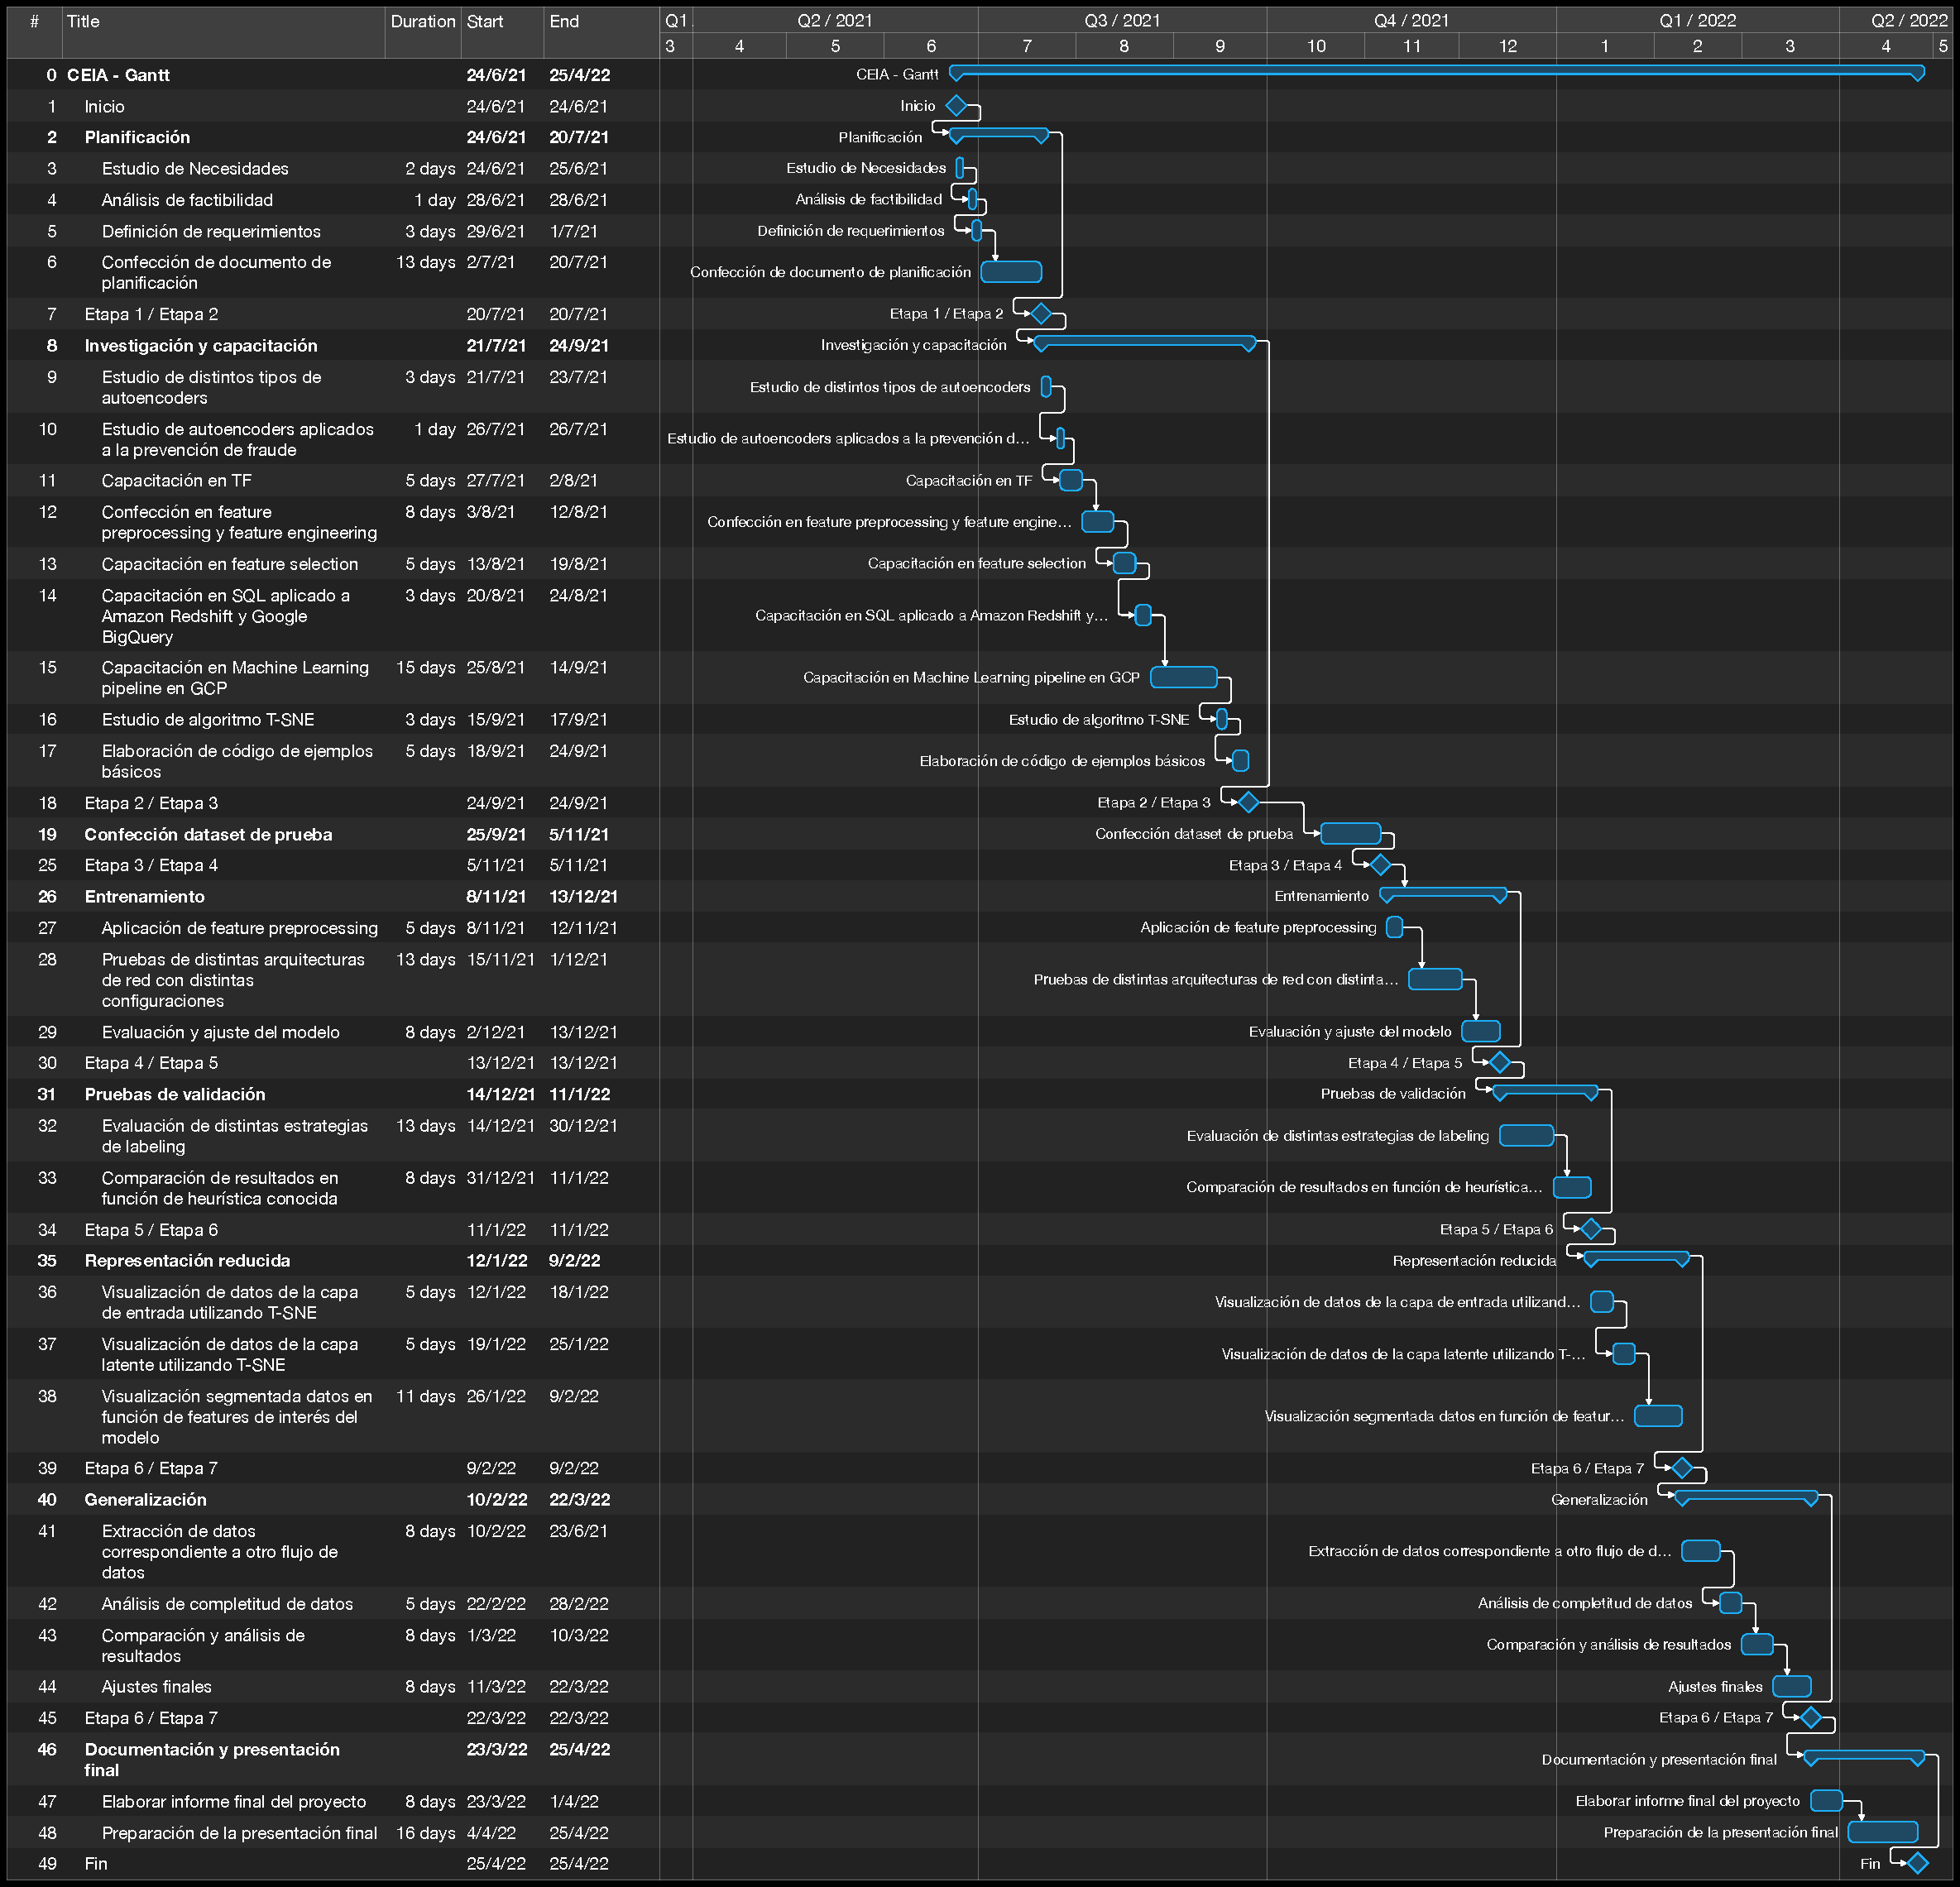
\includegraphics[width=\textwidth,  height=0.9\textheight]{./Figuras/ganttCompleto.pdf}
\caption{Diagrama de Gantt desglosado en tareas.}
\label{fig:ganttCompleto}
\end{figure}

\section{12. Presupuesto detallado del proyecto}
\label{sec:presupuesto}

En esta sección se detallas los gastos del proyecto. Las unidades del valor unitario están dadas en dólares estadounidenses.

Las cantidades del uso de los servicios son estimadas. En el caso de Amazon Redshift y Google BigQuery se ha considerado el gasto mensual fijo del uso del servicio que paga la empresa. En el caso de Amazon Redshift se ha estimado que se almacenará 1 Terabyte de información durante 10 meses. Finalmente, para el caso de entrenamientos, se ha considerado que los entrenamientos de los experimentos durarán 50 horas y tendrán lugar durante un mes.

\begin{table}[htpb]
\centering
\begin{tabularx}{\linewidth}{@{}|X|c|r|r|@{}}
\hline
\rowcolor[HTML]{C0C0C0} 
\multicolumn{4}{|c|}{\cellcolor[HTML]{C0C0C0}COSTOS DIRECTOS} \\ \hline
\rowcolor[HTML]{C0C0C0} 
Descripción &
  \multicolumn{1}{c|}{\cellcolor[HTML]{C0C0C0}Cantidad} &
  \multicolumn{1}{c|}{\cellcolor[HTML]{C0C0C0}Valor unitario} &
  \multicolumn{1}{c|}{\cellcolor[HTML]{C0C0C0}Valor total [USD]} \\ \hline
 	Mano de obra & 
  	\multicolumn{1}{c|}{600 horas} &
  	\multicolumn{1}{c|}{10 USD/hora} &
  	\multicolumn{1}{c|}{6000} \\ \hline
 	Google BigQuery &
  	\multicolumn{1}{c|}{1 mes} &
  	\multicolumn{1}{c|}{1700 USD/mes} &
  	\multicolumn{1}{c|}{1700} \\ \hline
 	Amazon Redshift &
  	\multicolumn{1}{c|}{1 mes} &
  	\multicolumn{1}{c|}{1380 USD/mes} &
  	\multicolumn{1}{c|}{1380} \\ \hline
 	Amazon S3 &
  	\multicolumn{1}{c|}{1 TB 10 meses} &
  	\multicolumn{1}{c|}{0.0.23 USD/GB/mes} &
  	\multicolumn{1}{c|}{235.52} \\ \hline
 	Google AI Platform &
  	\multicolumn{1}{c|}{1 mes} &
  	\multicolumn{1}{c|}{61.05 USD/mes} &
  	\multicolumn{1}{c|}{61.05} \\ \hline
\multicolumn{3}{|c|}{SUBTOTAL} &
  \multicolumn{1}{c|}{9376.57} \\ \hline
\rowcolor[HTML]{C0C0C0} 
\multicolumn{4}{|c|}{\cellcolor[HTML]{C0C0C0}COSTOS INDIRECTOS} \\ \hline
\rowcolor[HTML]{C0C0C0} 
Descripción &
  \multicolumn{1}{c|}{\cellcolor[HTML]{C0C0C0}Cantidad} &
  \multicolumn{1}{c|}{\cellcolor[HTML]{C0C0C0}Valor unitario} &
  \multicolumn{1}{c|}{\cellcolor[HTML]{C0C0C0}Valor total [USD]} \\ \hline
	30\% del costo directo & 
  	\multicolumn{1}{c|}{-} &
  	\multicolumn{1}{c|}{-} &
  	\multicolumn{1}{c|}{2812.97} \\ \hline
\multicolumn{3}{|c|}{SUBTOTAL} &
  \multicolumn{1}{c|}{2812.97} \\ \hline
\rowcolor[HTML]{C0C0C0}
\multicolumn{3}{|c|}{TOTAL} &
   \multicolumn{1}{c|}{12189.54} \\ \hline
\end{tabularx}%
\end{table}


\section{13. Gestión de riesgos}
\label{sec:riesgos}

\begin{consigna}{red}
a) Identificación de los riesgos (al menos cinco) y estimación de sus consecuencias:
 
Riesgo 1: detallar el riesgo (riesgo es algo que si ocurre altera los planes previstos de forma negativa)
\begin{itemize}
	\item Severidad (S): mientras más severo, más alto es el número (usar números del 1 al 10).\\
	Justificar el motivo por el cual se asigna determinado número de severidad (S).
	\item Probabilidad de ocurrencia (O): mientras más probable, más alto es el número (usar del 1 al 10).\\
	Justificar el motivo por el cual se asigna determinado número de (O). 
\end{itemize}   

Riesgo 2:
\begin{itemize}
	\item Severidad (S): 
	\item Ocurrencia (O):
\end{itemize}

Riesgo 3:
\begin{itemize}
	\item Severidad (S): 
	\item Ocurrencia (O):
\end{itemize}


b) Tabla de gestión de riesgos:      (El RPN se calcula como RPN=SxO)

\begin{table}[htpb]
\centering
\begin{tabularx}{\linewidth}{@{}|X|c|c|c|c|c|c|@{}}
\hline
\rowcolor[HTML]{C0C0C0} 
Riesgo & S & O & RPN & S* & O* & RPN* \\ \hline
       &   &   &     &    &    &      \\ \hline
       &   &   &     &    &    &      \\ \hline
       &   &   &     &    &    &      \\ \hline
       &   &   &     &    &    &      \\ \hline
       &   &   &     &    &    &      \\ \hline
\end{tabularx}%
\end{table}

Criterio adoptado: 
Se tomarán medidas de mitigación en los riesgos cuyos números de RPN sean mayores a...

Nota: los valores marcados con (*) en la tabla corresponden luego de haber aplicado la mitigación.

c) Plan de mitigación de los riesgos que originalmente excedían el RPN máximo establecido:
 
Riesgo 1: plan de mitigación (si por el RPN fuera necesario elaborar un plan de mitigación).
  Nueva asignación de S y O, con su respectiva justificación:
  - Severidad (S): mientras más severo, más alto es el número (usar números del 1 al 10).
          Justificar el motivo por el cual se asigna determinado número de severidad (S).
  - Probabilidad de ocurrencia (O): mientras más probable, más alto es el número (usar del 1 al 10).
          Justificar el motivo por el cual se asigna determinado número de (O).

Riesgo 2: plan de mitigación (si por el RPN fuera necesario elaborar un plan de mitigación).
 
Riesgo 3: plan de mitigación (si por el RPN fuera necesario elaborar un plan de mitigación).

\end{consigna}


\section{14. Gestión de la calidad}
\label{sec:calidad}

\begin{consigna}{red}
Para cada uno de los requerimientos del proyecto indique:
\begin{itemize} 
\item Req \#1: copiar acá el requerimiento.

\begin{itemize}
	\item Verificación para confirmar si se cumplió con lo requerido antes de mostrar el sistema al cliente. Detallar 
	\item Validación con el cliente para confirmar que está de acuerdo en que se cumplió con lo requerido. Detallar  
\end{itemize}

\end{itemize}

Tener en cuenta que en este contexto se pueden mencionar simulaciones, cálculos, revisión de hojas de datos, consulta con expertos, mediciones, etc.  Las acciones de verificación suelen considerar al entregable como ``caja blanca'', es decir se conoce en profundidad su funcionamiento interno.  En cambio, las acciones de validación suelen considerar al entregable como ``caja negra'', es decir, que no se conocen los detalles de su funcionamiento interno.

\end{consigna}

\section{15. Procesos de cierre}    
\label{sec:cierre}

\begin{consigna}{red}
Establecer las pautas de trabajo para realizar una reunión final de evaluación del proyecto, tal que contemple las siguientes actividades:

\begin{itemize}
	\item Pautas de trabajo que se seguirán para analizar si se respetó el Plan de Proyecto original:
	 - Indicar quién se ocupará de hacer esto y cuál será el procedimiento a aplicar. 
	\item Identificación de las técnicas y procedimientos útiles e inútiles que se emplearon, y los problemas que surgieron y cómo se solucionaron:
	 - Indicar quién se ocupará de hacer esto y cuál será el procedimiento para dejar registro.
	\item Indicar quién organizará el acto de agradecimiento a todos los interesados, y en especial al equipo de trabajo y colaboradores:
	  - Indicar esto y quién financiará los gastos correspondientes.
\end{itemize}

\end{consigna}


\end{document}
